\documentclass[conference]{IEEEtran}
\usepackage{fancyhdr}\usepackage[utf8]{inputenc}
\usepackage{graphicx}
\usepackage{multirow}

\usepackage{lastpage}
\usepackage{soul}

%\usepackage{draftwatermark}


%\SetWatermarkText{UoA}
%\SetWatermarkScale{3}

\pagestyle{fancy}
\fancyhf{}
\rfoot{Page \thepage \hspace{1pt} of \pageref{LastPage}} 

\title{Is it Possible to Extend IPv6?}
\date{December 2022}

\author{\IEEEauthorblockN{Ana Custura}
\IEEEauthorblockA{
\textit{University of Aberdeen}\\
}
\and
\IEEEauthorblockN{Raffaello Secchi}
\textit{University of Aberdeen}\\
\and
\IEEEauthorblockN{Gorry Fairhurst}
\textit{University of Aberdeen}\\
}
\begin{document}

\maketitle

\begin{abstract}
The IPv6 Hop-by-Hop Options and Destination Options Extension Headers have historically faced challenges in deployment due to a lack of router support coupled with concerns around potential for denial-of-service attacks. However, there has been a renewed interest within the standards community both in simplifying their processing, and in using these extension headers for new applications. 
Through a wide-scale measurement campaign, we show that many autonomous systems in both access networks and the core of the Internet do permit the traversal of packets that include options, and that the path traversal depends on the type of network, size of the option and the transport protocol used, but does not usually depend on the type of included option. This is an encouraging result when considering the extensibility of IPv6. We show that packets including extension headers can also impact the function of load balancing network devices, and present evidence of equipment mis-configuration, noting that a different path can result in a different traversal result. Finally, we outline the current deployment challenges and provide recommendations for how new options can utilise extension headers to extend IPv6.

\end{abstract}

\begin{IEEEkeywords}
IPv6 protocol, Extension Headers, Protocol Evolution, Destination Options, Hop-by-hop Options
\end{IEEEkeywords}

\section{Introduction}
\label{sec:introduction}

IPv6 Extension Headers (EHs)~\cite{RFC8200} are optional headers that a source node can
add following the base IPv6 header. They can be used to extend IPv6 by introducing new functionality and add features as a packet traverses a network path.  
%The use of extension headers allows for a flexible and extensible design of IPv6 that can support a variety of new networking features and technologies.
% commented out as it does not say much
IPv6 EHs are already widely used to implement specific functions (e.g., end-to-end use of IPsec, and use within a network to perform source routing).
In this paper we focus on network support for two EHs: the Destination Options (DST) header and the Hop-by-Hop Options (HBH) header~\cite{rfc9098}, as these are the primary means to introduce new end-to-end IPv6 functions.

Recent presentations to the networking community have commented on the limited
path traversal of packets including EHs and noted that network devices, such as
firewalls, routers, load balancers and intrusion detection
systems~\cite{nalini-iepg114, fernando-talk} do not properly handle packets
that include an EH. 
%These limitations can result in a packet drop (i.e., where a packet that
%includes an EH fails to traverse the end-to-end path).
Plausible reasons for the limited traversal are documented
in~\cite{ietf-v6ops-hbh-03}, where the authors note that early IPv6 routers
processed EHs in software. This processing typically utilises the slow-path,
rather than an optimised fast-path (e.g., using hardware forwarding), resulting
in a decreased router forwarding rate. In some designs, this processing
consumes Control Plane resources, opening-up a potential DoS attack vector on
the critical router functions (reducing ability to perform routing, management,
etc). This could have motivated network operators to implement policies that
drop packets that include EHs~\cite{rfc9098}.  To date this has discouraged use
of EHs. 

Additionally, some network administrators use firewalls to implement Access
Control Lists (ACLs) at the outer edge of access and enterprise networks, which
discard packets including an EH. This can mitigate security concerns, such as
bypassing security mechanisms or defending against denial-of-service (DoS)
attacks~\cite{naagas2021deh}, but also results in packet drop.

%XXX at some point here we will include a ref to ASIC XXX

The desire to add functionality motivates a fresh look at the usability of EHs
as a mechanism to extend IPv6: modern high-speed routers are being introduced
with flexible forwarding hardware capable of parsing and processing simple
headers within the fast-path~\cite{programmable-data-plane, cisco-silicon-one,
hauser2023}; and specific use-cases have emerged where there is an operational
demand for techniques that can be effectively implemented through EHs.  This
paper provides insight into whether these changes in operations and equipment
have impacted the forwarding of packets that include EHs, and seeks to
understand the opportunity to use these EHs to introduce new functions. 

The remainder of this paper is organised as follows:
Section~\ref{sec:background} presents the required background for IPv6 EHs and
describes the historical challenges related to their deployment.  The
literature describing measurement of paths is surveyed in
Section~\ref{sec:motivation}.
Section~\ref{sec:methodology}-\ref{sec:pathspider-results} presents our
methodology using a broad dataset to explore key aspects (e.g., the size of the
EH, the choice of transport, and choice and composition of the EH Options),
revealing a more diverse and nuanced picture of Internet paths than was
previously reported. The results are organised by the type of network path and
the analysis provides insight into why previous independent measurements
reported a variety of results ~\cite{RFC7872} \cite{apnic}
\cite{nalini-iepg114} \cite{james}.  The implications of our results are
discussed in Section~\ref{sec:discussion}, along with recommendations for how
these might in future be utilised.  Finally, the conclusion summarises our
findings, and seeks to answer the question about whether EHs can be used to
extend IPv6.


\section{Extending IPv6}
\label{sec:background}

%%XXX EH or OPT????????

\label{sec:ipv6-option-deployment}

\begin{figure}
\centering
  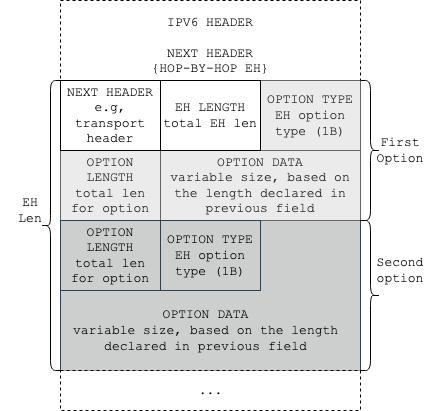
\includegraphics[width=0.5\textwidth]{ehformat.png}
  \caption{IPv6 packet with a base header that includes two EHs}
  \label{fig:eh-format}
\end{figure}

The IPv6 specification~\cite{rfc2460} introduced a flexible header structure
consisting of a fixed-length base header followed by one or more optional EHs.
When standardised, it was assumed that all routers would process an EH.
Initially, relatively few options were standardised and deployed.  When IPv6
became a full standard in 2017~\cite{RFC8200}, the processing rules for EHs were
modified to align with the prevailing operational practices at that time.

The Next Header field of the IPv6 base header indicates whether a packet
includes an EH.  Besides HBH and DST, IPv6 specifies EH for Routing, Fragment,
Authentication and Encapsulating Security Payload (ESP) header.  The Fragment
header, Authentication and ESP header operate end-to-end and follow the Routing
header, if present.  Each consecutive EH contains a Next Header field to
specify the type of the following EH, forming a chain terminated by the IPv6
payload. Each EH also contains a Length field specifying its length.  IPv6
~\cite{RFC8200}, does not specify a maximum size of the EH chain, but does
require it to be less than the first fragment in the case of fragmentation. 

When a HBH EH is included, it must be placed immediately after the base
header~\cite{RFC8200}.  Figure~\ref{fig:eh-format} shows the structure of an
IPv6 packet including a base header followed by a HBH EH containing two
Options.  A Routing EH (RH) can follow the HBH EH, e.g., to perform Source
Routing (SRv6). This is used  to ensure a path includes specified intermediate
routers, typically within a single domain~\cite{srv6}~\cite{srperf}. The DST EH
is placed immediately prior to the payload. This EH is permitted to be included
more than once (i.e.,  before the Routing EH or before the payload).  A HBH (or
DST)  before a Routing EH, has to be processed or skipped when a router is an
SRv6 intermediate nodes, to allow them to update the next destination in the
SRv6 header.  The DST and HBH EHs are the primary means by which IPv6 functions
can be extended, by introducing new options. 

Extension Headers contains Options encoded using a Type-Length-Value (TLV)
encoding~\cite{RFC8200} with 1~byte for each of the Type and Length fields, and
a variable-sized Value field that carries the option data. The total option
length must be a multiple of 8 bytes to guarantee alignement in router memory.
A router can skip any Option that does not recognise or is not configured to
support within an EH.  The two most significant bits (MSB) of the Type field specify
the action for an unrecognised header.  When set to "00", a router should
ignore the option and continue processing the header.  If the bits are
non-zero, the packet should be discarded.  When the bits are set to "01", an
ICMP message is returned to the sender. Similarly, if the bits are set to "11",
an ICMP message is sent, but only if the destination address is not multicast.

Table~\ref{tbl:options} presents the currently standardised Options.  Note that
most Options set the two MSBs to "00".

Setting the third MSB allows the data field of an Option to be modified by
routers on the path. Updating the contents of an Option can be used, for
example, to provide and collect data for traffic measurement
purposes~\cite{rfc9268}\cite{rfc9343}) or collect perational and telemetry
data using the recently-proposed Option 0x31.  Originally, all routers on a
path were required to examine and process the HBH EH~\cite{rfc2460}. This
requirement was relaxed by~\cite{RFC8200} to only require processing when
support is configured, e.g., option 0x0F~\cite{rfc8250} can be used to measure
performance and provide diagnostic metrics such as round-trip delay. 

% The total EH length is 8-byte aligned and specified in the
% EH Length field, while each individual option declares its own length in the
% Option Length field. 

\begin{table}[b]
\center
\caption{Currently Standardised DST and HBH Options.}
\begin{tabular}{p{0.03\textwidth}|p{0.055\textwidth}|l|p{0.18\textwidth}}
Hex  & MSBs & Type      & Description                                              \\
\hline
\hline
0x00 & 000  & HBH, Dest & Pad1 (padding)                                           \\
0x01 & 000  & HBH, Dest & PadN (padding)                                           \\
0xC2 & 110  & HBH       & Jumbo payload                                  \\
0x23 & 001  & HBH       & Low-Power and Lossy Networks Routing                     \\
0x04 & 000  & Dest      & IPv6 Encapsulation                 \\
0x05 & 000  & HBH       & Router Alert Option         \\
0xC9 & 110  & Dest      & Mobility Support in IPv6                                 \\
0x8C & 100  & Dest      & Identification of Broadband Subscribers\\
0x6D & 011  & HBH       & Multicast Protocol for Low-Power and  Lossy Networks     \\
0x0F & 000  & Dest      & Delay Measurement                                        \\
0x30 & 001  & HBH       & MinPathMTU                                     \\
0x11 & 000  & HBH, Dest & \multirow{2}{*}{On-path Operational Info}                \\
0x31 & 001  & HBH, Dest &                                                          \\
0x12 & 000  & HBH, Dest & On-path Telemetry                                       
\end{tabular}
  \label{tbl:options}
\end{table}


\subsection{Previous Path Traversal Studies for IPv6 with EHs}

\label{sec:motivation}

The Internet community has long been aware of the limited traversability faced
by packets containing EHs.  In 2015, an Informational IETF RFC presented
traceroute measurements to destinations within the Alexa top 1M
domains~\cite{RFC7872} and revealed a significantly higher drop rate for
packets that include EHs over the Internet compared to packets without EHs.
Other studies~\cite{james}~\cite{nalini-iepg114}~\cite{apnic} have also
supported this claim.  However, the level and nature of the loss figures varied
significantly from report to report. This motivated further analysis and
different investigation methods to understand the causes of this loss
~\cite{james}~\cite{elkins-v6ops-eh-deepdive-fw-01}).  

Another IETF draft, ``Just Another Measurement of Extension header
Survivability" (JAMES)~\cite{james}, presented results using traceroute over a
mesh network with 21 vantage points located in a set of globally distributed
Autonomous Systems (ASes). This study tested all standard EHs in a setting
where both endpoints are under the control of the researcher concluding that
only 8-9\% of paths in Internet can be traversed by an 8-bytes HBH EH, and a
97\% traversal for an 8-bytes DST EH.  These traversal ratios decrease as the
size of the EH increases~\cite{james-imc}. It should be noted, however, that 6
of the 21 vantage points were hosted by Digital Ocean\texttrademark, an
Internet service provider that drops packets including HBH EHs.

An innovative measurement methodology was proposed by engineers in
APNIC~\cite{apnic} to analyse end-to-end traversal for Fragmentation, HBH and
DST EHs.  This technique consists in opening TCP connections using IPv6 packets
with EHs from a crowd-sourced pool of clients and evaluating the number of
successful connection establishments.  APNIC reported results from 4M
measurements/day from clients across the Internet.  It was found that 50\%  of
attempts to open a connection with a DST EH was successful but close to 0\%
when a HBH EH was included.  It should be noted, however, that this test
required both the Internet path to support the EH and the endpoint to reply to
a packet that included an Option. 

%\hl{XXXX These results were updated in 2023 (using a server co-located with a
%measurement server used in the analysis described in the next section) and
%reported XXXX}.  We also note that all measurements were performed from
%servers in a single Cloud provider (Linode).

% The different results outlined above present conflicting views, representative
% of the complex nature of Internet paths. We argue the differences are explained
% by examining the types of networks measured and the choice of vantage points
% and destinations. To fully explore the various aspects of EH traversal, our
% work takes a large-scale measurement approach, testing a wide range of access,
% core and server edge networks, and focuses on the HBH and DST EH types.
% In Section~\ref{sec:discussion}, our results from measurements in access
% networks are compared and discussed alongside their closest counterpart - the
% measurements presented in JAMES~\cite{james}. As we also test edge paths to
% target servers based on top 1M domains lists, we refresh the data presented
% in~\cite{RFC7872} for a longitudinal view.

A large-scale passive measurement campaign used the Czech Republic national
research and education network to analyse IPv6 traffic over a period of one month in
2016~\cite{passive-threats}. It found that 0.1\% of IPv6 flows
that include an EH, out of which 40.9\% packets included HBH with an ICMPv6
payload, this was primarily multicast (although not specified by the original authors,
we identify this as Multicast for Low-Power and Lossy Networks~\cite{RFC7731}).
The study also noted that dropping of ICMPv6 traffic that include EHs could result in
loss of essential network control information. 

% With the exception of~\cite{james-imc}, there are no other peer-reviewed active
% measurement studies. 

Our large-scale measurement study complements and extends these previous analyses. It not only
looks at the end-to-end support in servers, but also provides comparative path
analysis and observation of longitudinal changes in the traversal for HBH and DST.

\subsection{Challenges and Operational Considerations}


The Internet hosts a wide range of router designs, spanning from Customer
Premises Equipment (CPE) access routers to high-speed transit routers with the
capacity to handle thousands of GB/s.  Many high-speed routers use an
architecture where packets are processed on the ``fast-path" utilising hardware
support (e.g., an Application Specific Integrated Circuit, ASIC). Packets that
cannot be processed on this path use the ``slow-path" in software, possibly
using the control plane processor~\cite{RFC3654} ~\cite{ietf-v6ops-hbh-03}.
Using the slow-path exposes the routers to DoS (Denial of Service)
attacks~\cite{naagas2021deh}, where traffic processing is forced on the control
plane reducing resources to manage the router~\cite{router-architecture}. This
could be mitigated  by reducing the rate of packets entering the control plane.
According~\cite{passive-threats}, awareness of this problem motivated network
operators to configure routers to discard packets that include an EH, in
particular HBH EHs. These authors also noted that some routers discard packets
including EHs due to flawed implementations of the IPv6
stack~\cite{passive-threats}.  This paper aims to analyse whether this practice
remains prevalent in the current Internet and thus continues to pose an
obstacle to EH deployment.

Certain network nodes also have a need to inspect the transport protocol
information, for instance when an Access Control List (ACL) inspects the ports.
Use of ACLs is common at a network domain edge, including the edge of enterprise
and home access networks, e.g. to implement firewalls, multi-field QoS
classifiers, deep packet inspection (DPI) and DoS attack
mitigation~\cite{lb-classification}. Some access-network routers also modify
upper layer protocol headers to avoid issues related to encapsulation, e.g.,
by performing TCP Maximum Segment Size (MSS) Clamping~\cite{custura-mtu}. When
an EH is present, the router must parse the entire IPv6 header
chain and locate the payload and modify the TCP header. 

Routers that operate in transit networks typically do not require access to
upper-layer information. A notable exception are the devices performing Equal
Cost Multipath Routing (ECMP) or application-layer load balancing that can use
transport-layer information to improve utilisation on multiple alternative
paths. RFC 9288~\cite{rfc9288} recommends that transit routers forward packets
only on the fast-path, or employ a mechanism to limit the rate of packets
appearing on the slow-path.  Whenever no rate mitigations are available over
the slow-path, discarding packets is recommended. 

%In the early Internet, packet routers were implemented entirely
%in software, and as the Internet grew packet processing was moved from software
%to Application Specific Integrated Circuits (ASICs), while the control
%functions remained~\cite{router-architecture}. Routers started having a split
%architecture with a control and forwarding plane~\cite{RFC3654}, corresponding
%to router-critical operations running in software and hardware processing
%respectively. 
%In this architecture, incoming packets can be processed on the
%``fast-path" in the forwarding plane on an ASIC or sent for processing over an
%internal link on the ``slow-path", or the control plane of a router. 

%As IPv6 emerged, ASIC support for it was limited, and IPv6 deployment itself was in its infancy - and many network router architectures processed packets containing IPv6 EHs in software~\cite{ietf-v6ops-hbh-03}.  This resulted in opening these routers up to DoS attacks~\cite{naagas2021deh}, because clients sending a large amount of IPv6 traffic including EHs could affect a router's control plane functions where no rate-limiting of such packets was available. This steered
%network operators to configure their routers to discard packets containing EHs,
%in particular the HBH EH~\cite{ietf-v6ops-hbh-03}.

%https://ieeexplore.ieee.org/stamp/stamp.jsp?tp=&arnumber=7949061

%\subsection{Hop-by-Hop and Destination Option EHs}

%An IPv6 packet can contain zero or more EHs, each identified by its own number
%in the Next Header field in the preceding header. The HBH header is
%indicated by the value 0, while the assigned protocol number for the DST
%header is 60. Both HBH and DST can be included in the same IPv6 packet in
%different EHs. An EH can contain multiple Options - Figure~\ref{fig:eh-format}
%presents one EH including 2 Options.


% Although intended to be
% processed differently, HBH and DST EHs carry a variable number of Options
% that share the same Type-Length-Value (TLV) encoding~\cite{RFC8200}. Option
% Type and Length are each encoded within one Byte, followed by a variable-size
% Option Value field that carries the option data. Figure~\ref{fig:eh-format}
% shows this format. The total EH length is 8-byte aligned and specified in the
% EH Length field, while each individual option declares its own length in the
% Option Length field. Standardized option types are presented in
% Table~\ref{tbl:options}.

% Please add the following required packages to your document preamble:



%\subsection{Operational considerations}


\section{Description of Datasets} 
\label{sec:methodology}

This paper employs a combination of tools and experiments to explore HBH and
DST EHs traversal (see Table~\ref{tbl:datasets}). The setup for each test is
discussed in the next subsections.

\begin{table}
\caption{Experiments and Datasets}
\begin{tabular}{p{0.17\textwidth}|p{0.075\textwidth}|p{0.03\textwidth}|p{0.065\textwidth}|p{0.03\textwidth}}
Purpose                                                                          & Tool         & Name & Date               & Trans. \\
\hline
\hline
Test traversal of 8~B Opts in access networks             & Traceroute       & R1           & Oct 2022- Jan 2023 & UDP TCP          \\
\hline
Test traversal and EH size in access networks           & Traceroute       & R2           & Oct 2022           & UDP TCP          \\
\hline
Test whether a consistent path is used 			& Paris Traceroute & R3           & Jan 2023           & UDP               \\
\hline
Explore traversal of Opts to the server edge              & PATHSpider       & P1           & Jul 2020- Jan 2023 & UDP TCP          \\
\hline
Explore variations in Opt type, length or content        & PATHSpider       & P2           & Jul 2022- Dec 2022     & UDP              
\end{tabular}
  \label{tbl:datasets}
\end{table}
    
\subsection{Access network paths using RIPE Atlas}
\label{sec:ripe-methodology}

Datasets R1-R3 in Table~\ref{tbl:datasets} were collected using the RIPE Atlas
measurement platform~\cite{bajpai2015lessons}.  This platform provided 5464
IPv6 vantage points (probes) across 644 unique AS Numbers (ASNs), spanning a
range of commercial ISPs and R\&E access networks.  
% The number of actual available probes fluctuates because it relies on
% volunteer-run probes in edge networks that can be disconnected. 
Packets were sent with a PadN Option inserted in a DST and HBH EH. This Option
was defined in the original IPv6 standard to provide 8~B alignment within an EH
and is expected to be safely recognised by all IPv6 implementations.  

Data was collected using both UDP and TCP transports from multiple vantage
points, targeting seven globally distributed servers (dataset R1).  In a
separate experiment (dataset R2), the destination country remained fixed while
varying the transport and EH size from 8B to 64B.


Finally, we used Paris Traceroute~\cite{augustin2006avoiding}, to detect
whether the presence of an EH influences the path taken. In this case, we only
selected vantage points where traversal was successful over UDP for both types
of tested EH to a specific target, resulting in a total of 866 measured paths.
We measured these paths using IPv6 packets with no EH, and packets carrying 8~B
DST and HBH EHs. Each measurement was repeated 16 times (each identified by  a
Paris ID), as in~\cite{augustin2006avoiding}. Each repetition varied the source
port and the Flow Label  The set of  measurements was repeated 5 times (dataset
R3).

\subsection{Measuring server edge paths using PATHSpider}
\label{sec:pathspider-methodology}

Additional tests were conducted using
PATHSpider~\cite{learmonth2016pathspider}, a path transparency testing tool.
These tests surveyed IPv6-enabled Domain Name System (DNS) servers over
multiple years (2019-2023) from the University of Aberdeen vantage point.
The experiment targeted IPv6 authoritative Name Servers (NS) for the
then-current Alexa Top 1M domains list. The longitudinal measurement focused on
UDP results, using a consistent set of domains to avoid list changes. Each
domain was resolved, removing duplicates and unreachable addresses, resulting
in 19,000 - 22,000 unique IPv6 addresses per test.


PATHSpider was extended to support TCP measurements. In 2023, UDP and TCP
transports were used from five global vantage points to test DNS and web
servers extracted from the Cisco Umbrella Top 1M Domains. ICMP message
reception was also recorded to analyze router behavior with EH packets.

%We extended PATHSpider to support measurements over TCP and then repeated this
%test in 2023 using both UDP and TCP transports from 5 globally distributed
%vantage points to both DNS and web servers extracted from the latest version of
%Cisco Umbrella Top 1M Domains (19,054 and 232,350 unique IP addresses
%respectively). When TCP is measured, the EH is included on the first (the TCP
%SYN) and all subsequent packets in the connection.  This test also records
%whether any ICMP messages are received, to understand whether routers are
%configured to send ICMP messages when they drop a packet with an EH.


In the subsequent experiment (dataset P2), we explored the effects of varying
the Option Type and Option Length fields. The objective was to observe how
different types of options, as well as incorrectly declared lengths, impact
traversal. Additionally, we recorded any received ICMP messages for each
source-destination pair to determine the frequency of ICMP Type 3 (Destination
Unreachable) or ICMP Type 4 (Parameter Problem) messages sent by routers when
dropping packets. It is important to note that this test ensures one tested
Option Type has the highest order bits set to 11, as indicated in
Table~\ref{tbl:options}.

%In the next experiment, we vary the Option Type and the Option Length fields
%(dataset P2) to observe whether different types of Options, or an incorrectly
%declared length affects traversal and record any ICMP messages received for a
%source-destination pair, to understand how often ICMP Type 3 (Destination
%Unreachable) or ICMP Type 4 (Parameter Problem) messages are sent by routers
%when they drop packets. This test ensured one tested Option Type has the
%highest order bits set to 11 (see Table~\ref{tbl:options}.

For the server-side measurements, the selected targets are DNS servers, which
allows these to be surveyed using both UDP and TCP, although we also present
traversal results for the web servers underpinning the Cisco Umbrella top 1M
domains.

% The next two sections present results for the Atlas Platform (the access
% network) and for PATHSpider (at the server edge).


\section{Measurement Results using RIPE Atlas Probes} 
\label{sec:ripe-results}

\begin{figure}[t]
\centering
  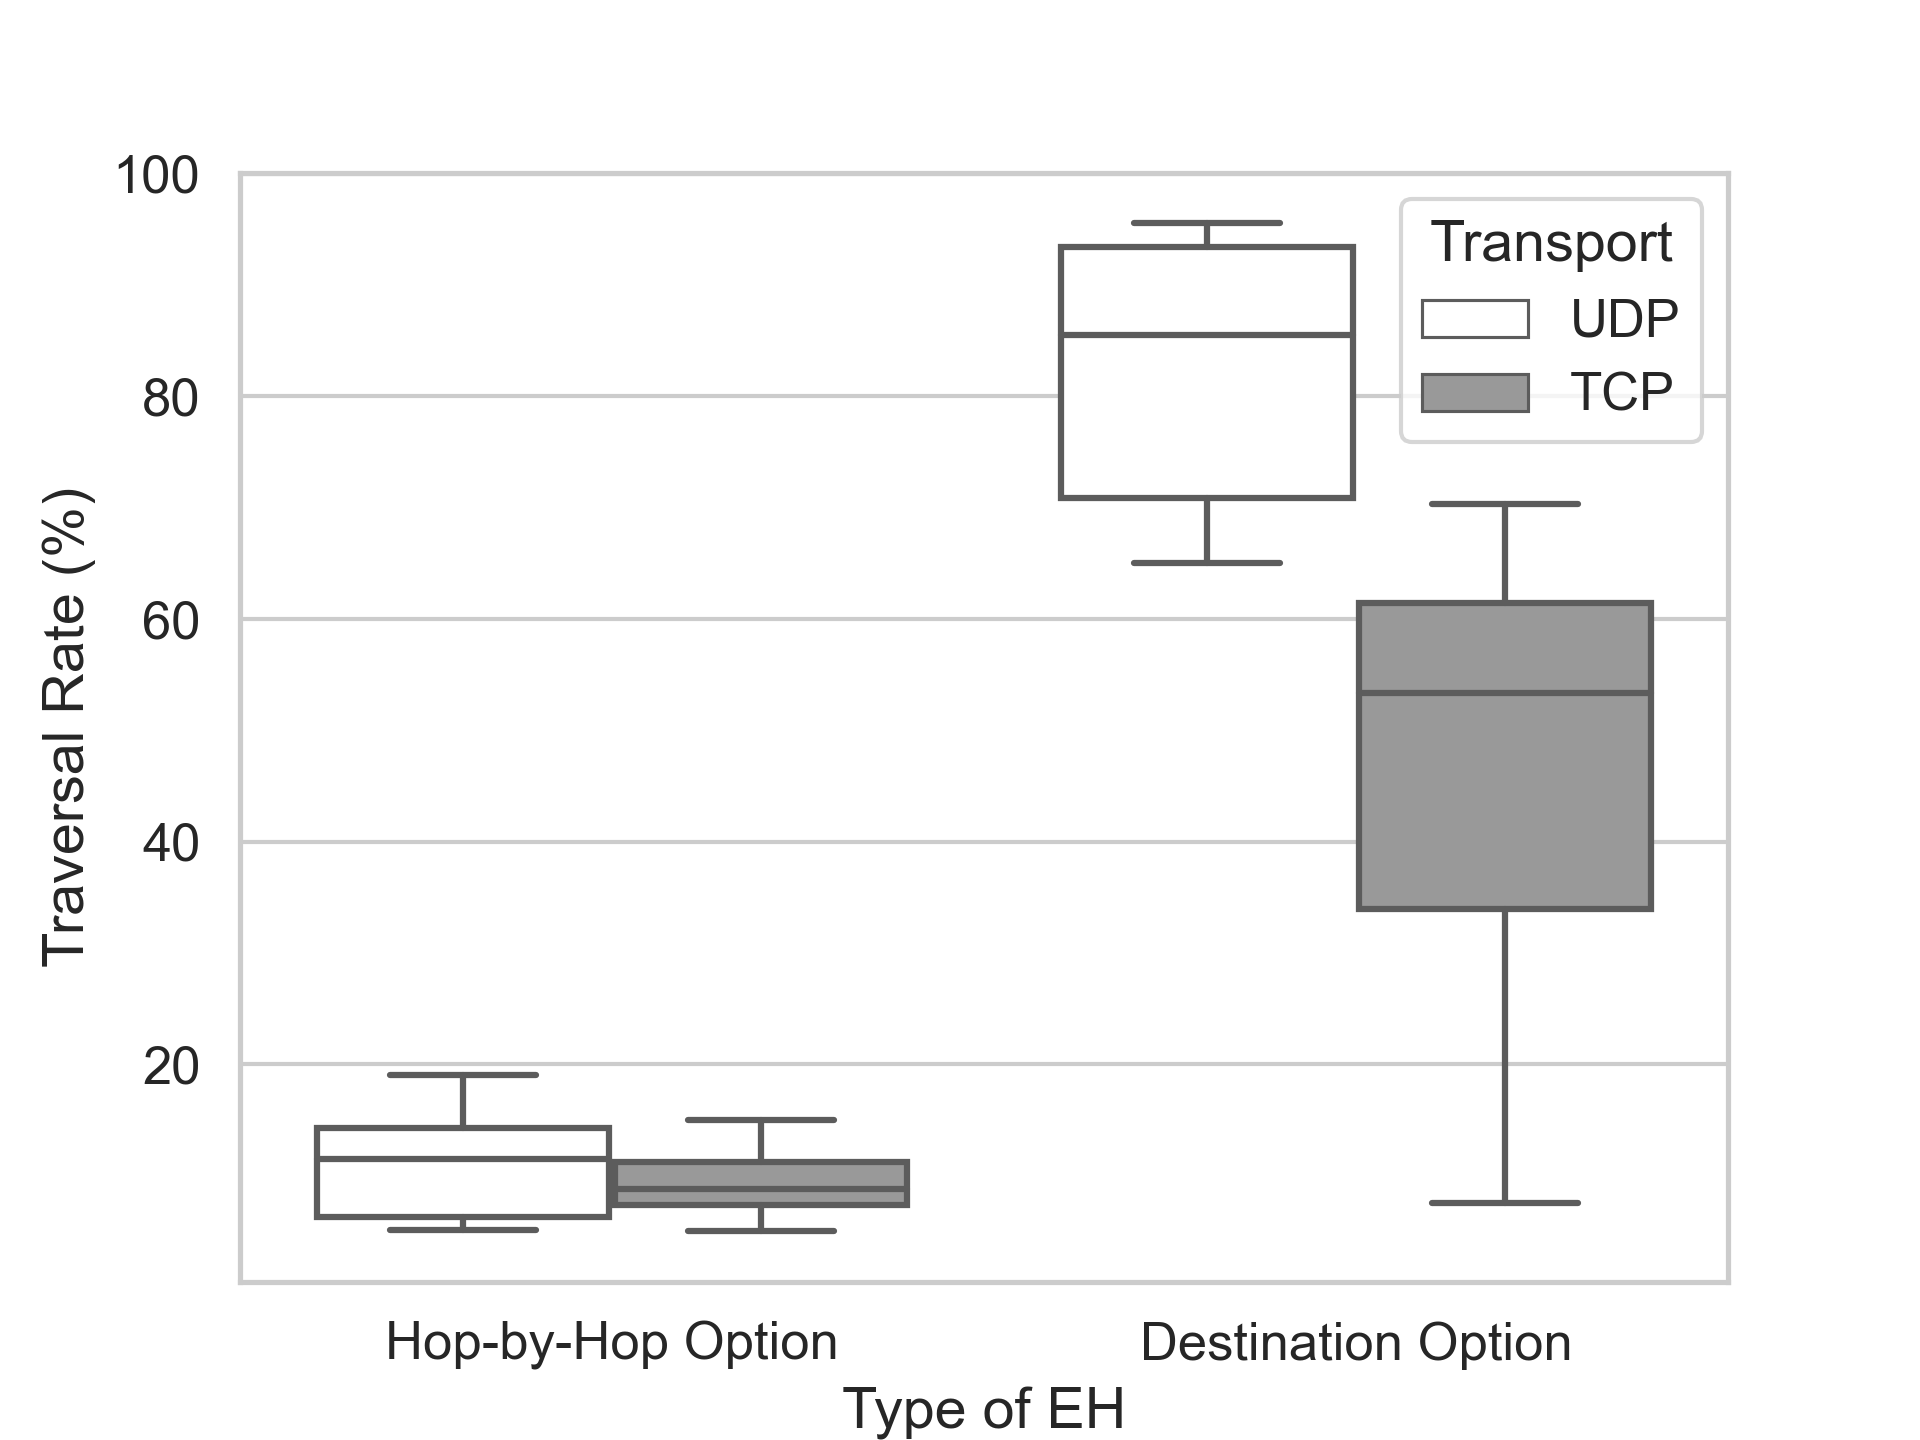
\includegraphics[width=0.5\textwidth]{all_traversal.png}
  \caption{Traversal for packets including HBH and DST, from Atlas vantage points to target servers located in 7 different countries (dataset R1).}
  \label{fig:countrybox}
\end{figure}

In this section, we present the results conducted on the Atlas platform. 
The primary performance metric analysed is the "traversal ratio",
which represents the proportion of paths where probe packets with EHs
successfully reached the destination AS compared to the total paths tested.
This section also discusses the pathologies associated with the most
critical destinations.

\subsection{Traversal Ratio to Destination AS}

%Prior to each test case, a baseline measurement using vanilla packets was
%carried out and unreachable probes were subsequently removed from the result
%set. 

Figure~\ref{fig:countrybox} shows the distribution of the traversal ratio with
four transport header compositions (using DST or HBH extension headers, and
using TCP or UDP), while consistently employing the PadN Option in EHs.  The target
destinations were located in seven countries (the United States (US), the
United Kingdom (UK), Australia, Poland, Zambia, Kazakhstan, and Singapore) using
an average of 4750 vantage points per destination.

The figure shows a 83\% and 57\% median for path traversal 
respectively using a packet that includes the
DST EH and carries a UDP and TCP payload.  The traversal ratio is lower
for a HBH EHs, with a median of 12\% (UDP) and 9\% (TCP). The traversal ratio
 for TCP has much greater variability than with
UDP, ranging from 8\% for Zambian destinations to 67\% for destinations in the
UK. The lower traversal for HBH EHs, and for packets carrying TCP
was  linked to the
behaviour and configuration of routers within access networks, more
specifically ISP ingress routers.

To understand the impact of EH size on the traversal ratio, we sent packets
 with an EH from 16~B to 64~B in 8-byte
increments from the ATLAS
vantage points to a server located within the UK's academic network
(JANET).  This experiment was repeated with
HBH and DST EHs, and using both UDP and TCP and preserved the alignment (dataset R2).


\begin{figure}[t]
\centering
  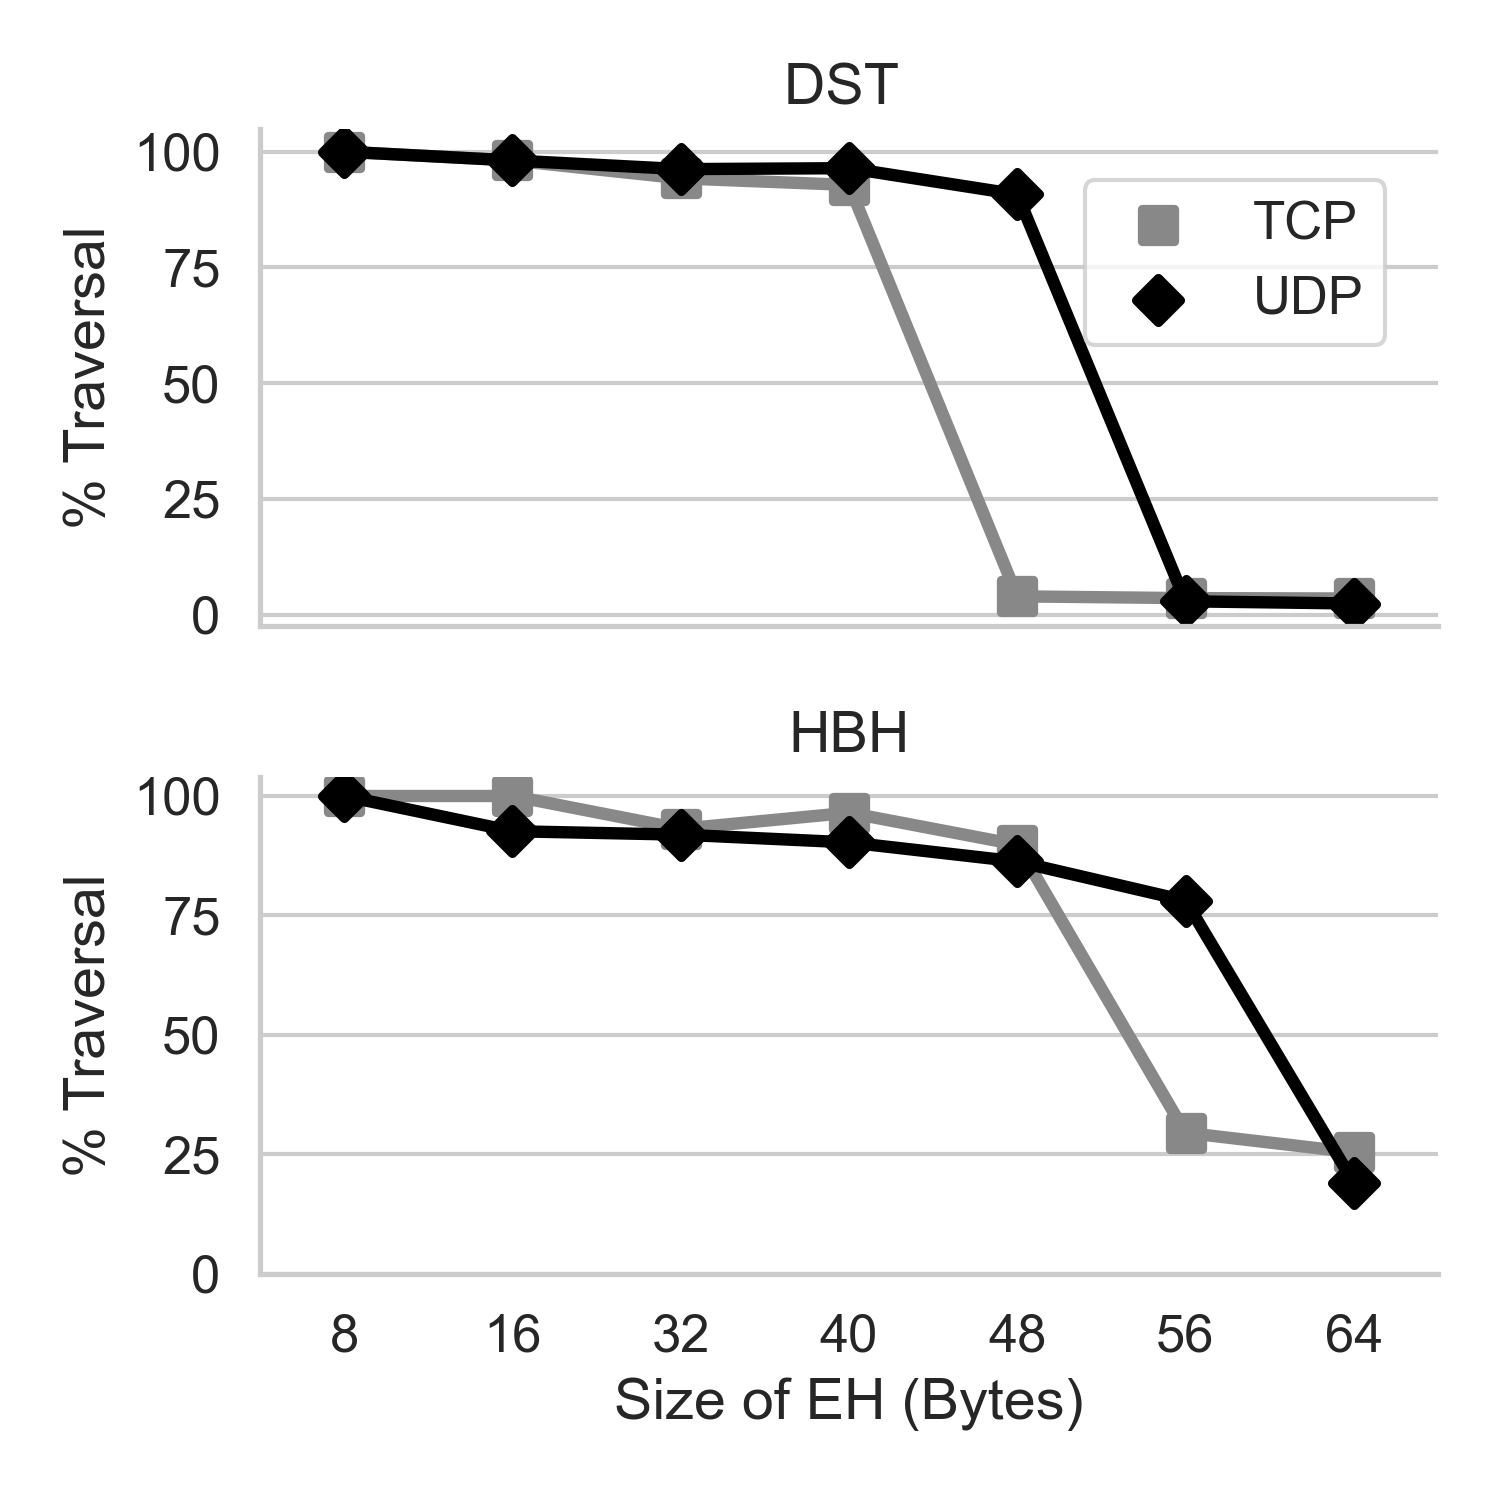
\includegraphics[width=0.45\textwidth]{sizes.png}
  \caption{Traversal ratio for packets including HBH and DST EHs from the Atlas
vantage points to a target server in the JANET network (AS876), showing
size of EH and split by transport.  Total n=129,585 measurements, with a mean
of 4628 measurements ($\sigma$=351) for each combination of transport, size and
EH (dataset R2). The variation in the number of measurements results from
availability and connectivity of  probes with time.  }

  \label{fig:sizes}
\end{figure}
 

The results depicted in Fig.~\ref{fig:sizes} show the relationship between
header size and traversal ratio, demonstrating a decrease in the traversal ratio
as the header size increases.  Packets containing a DST EH over UDP have the
most substantial decrease in traversal between 48B and 56B. The 
traversal ratio (2\%) is reduces for the same size for HBH EH. A
comparable pattern is observed in the TCP experiments, where the most significant
drop occurs between 40~B and 48~B.

%, because the header is 8~B smaller for UDP. --- eh? TCP=20B ; UDP = 8~B

The difference in traversal ratio between UDP and TCP is due to the overall
size of the transport header.  The combined header size of TCP (20~B) and IPv6
(40~B) with a 48~B EH is 108~B, while the combined header size of UDP and IP
with a 56~B EH is 104~B. This is consistent with a router parsing buffer of approximately 104~B
(see similar conclusions in ~\cite{james-imc}). These findings
resemble the reported results~\cite{james-imc}, which examined traversal
 for DST EHs of sizes 32B and 64B, and identified a lower traversal for
packets that include an EH larger than 64~B EH.
Although the size of the parsing buffer could increase with time, the size in deployed routers imposes a
constraint on the current usability of a large IPv6 EH.


%%% this size is strictly less than the size of the end-host parsing buffer
%[ref?]

\begin{figure}
\centering
  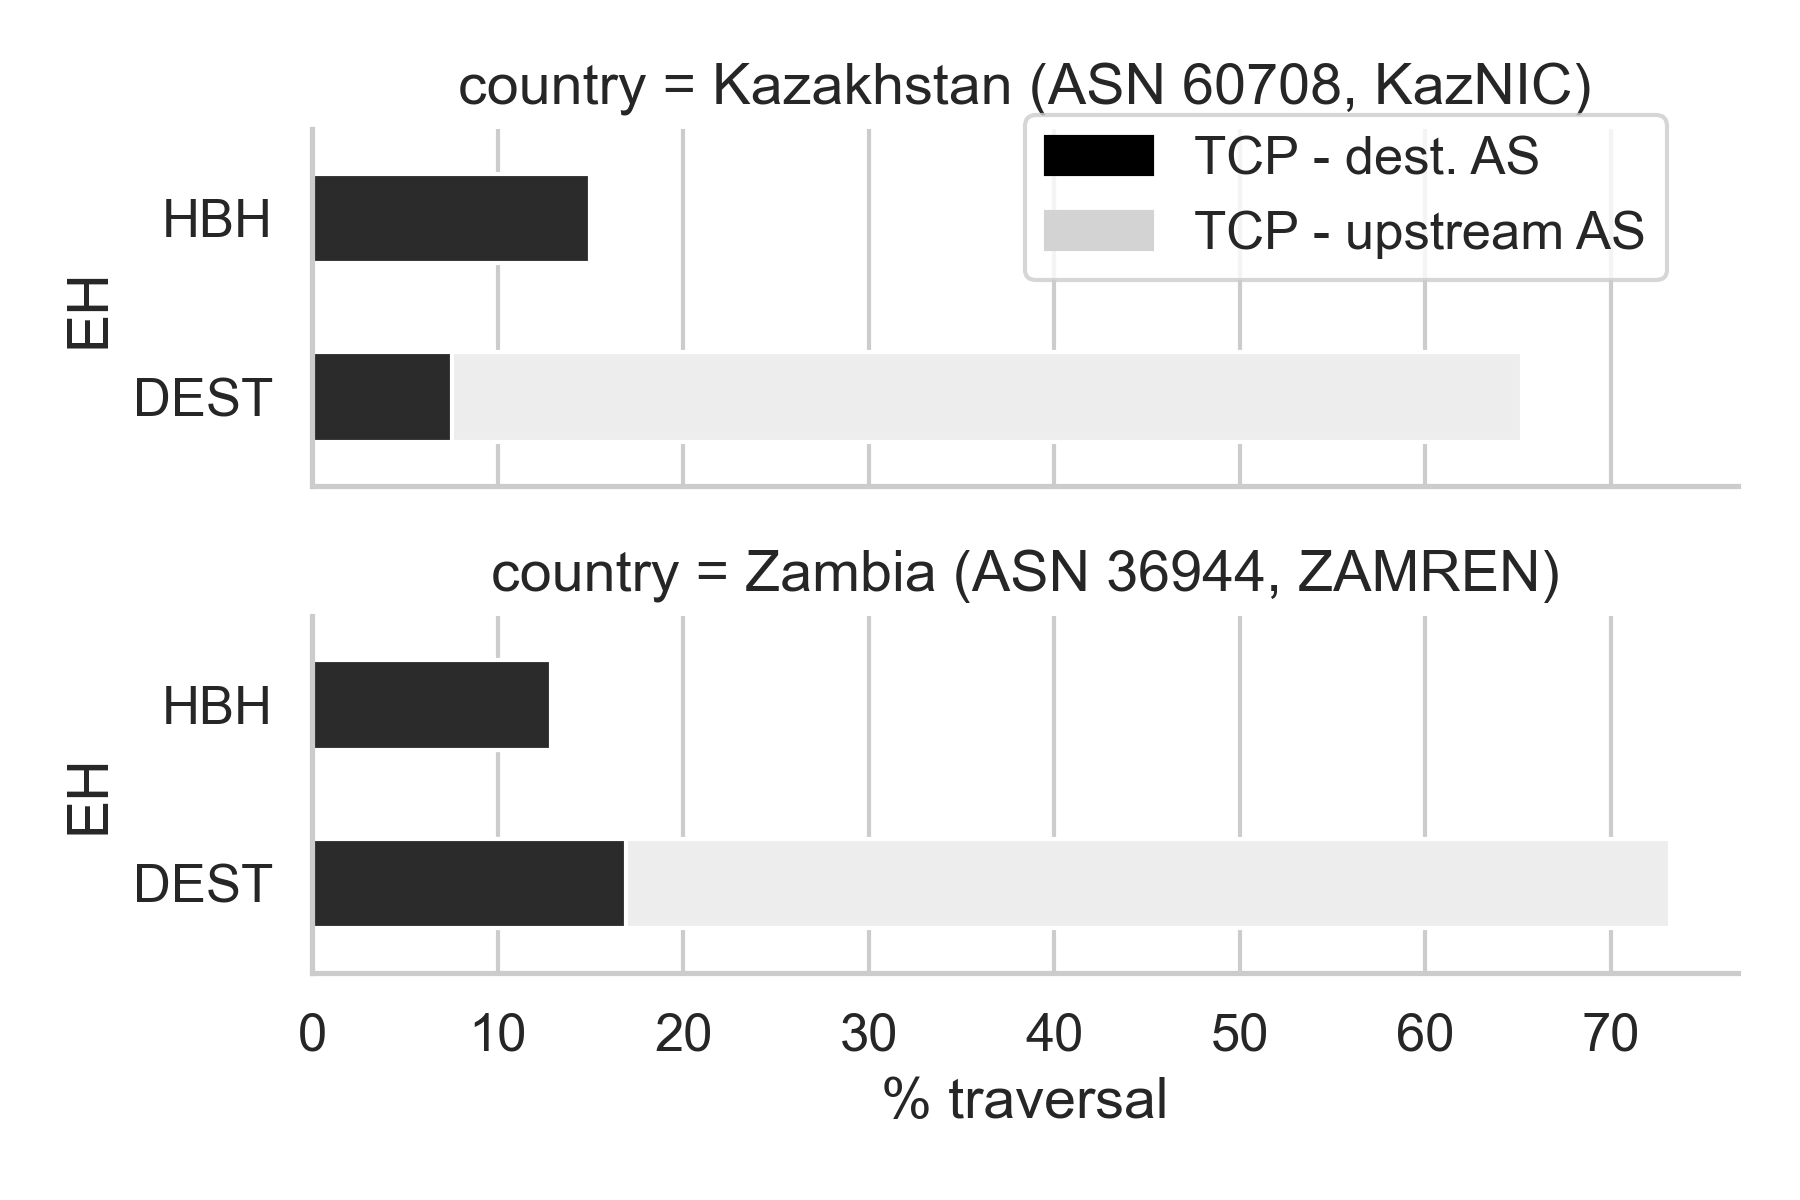
\includegraphics[width=0.5\textwidth]{traversal-pathologies.png}
  \caption{Packet traversal ratio for TCP payloads from Atlas vantage points to both destination and upstream
AS for targets in Kazakhstan (n=5075) and Zambia (n=4462).}
  \label{fig:traversal_pathologies}
\end{figure}

\subsection{Locating the Point of Drop Along the Path}

While there has been prior data on path traversal, less attention has been
given to identifying the specific router responsible for packet drops along the
path.

%We divide the path into the set of ASes.
Table~\ref{tbl:uk_as1} presents the traversal ratio along a
path, starting from an ATLAS vantage point towards a UK destination.
Within this table, the columns labelled as $1^{st}$, $2^{nd}$, and $\infty$
represent the traversal ratio within the first, second, and last AS.
Additionally, the columns labelled $1^{st}\rightarrow 2^{nd}$ and
$2^{nd}\rightarrow 3^{rd}$ indicate the traversal ratio at the peering point
between ASes.

\subsection{Drops within the First AS}

In mosts cases, a packet with a HBH EH sent from a vantage point that
includes an EH is dropped within the first AS  (68\% UDP, 74\% TCP).
Similarly, a notable fraction of DST EHs (5\% UDP, 25\% TCP) are dropped within the
initial AS, i.e.  within the AS where the vantage point is located, including
the first hop router. This drop rate is irrespective of the destination.
As we examine a path deeper in the network, the average probability of traversal
either remains the same, or decreases. 
UDP packets that include a DST EH
experience less than 1\% drop rate as they travel across further ASes.  This
suggests that, once the first AS is traversed, the packets with an EH travel to the
destination with minimal disruption.

\begin{figure}[t]
\centering
  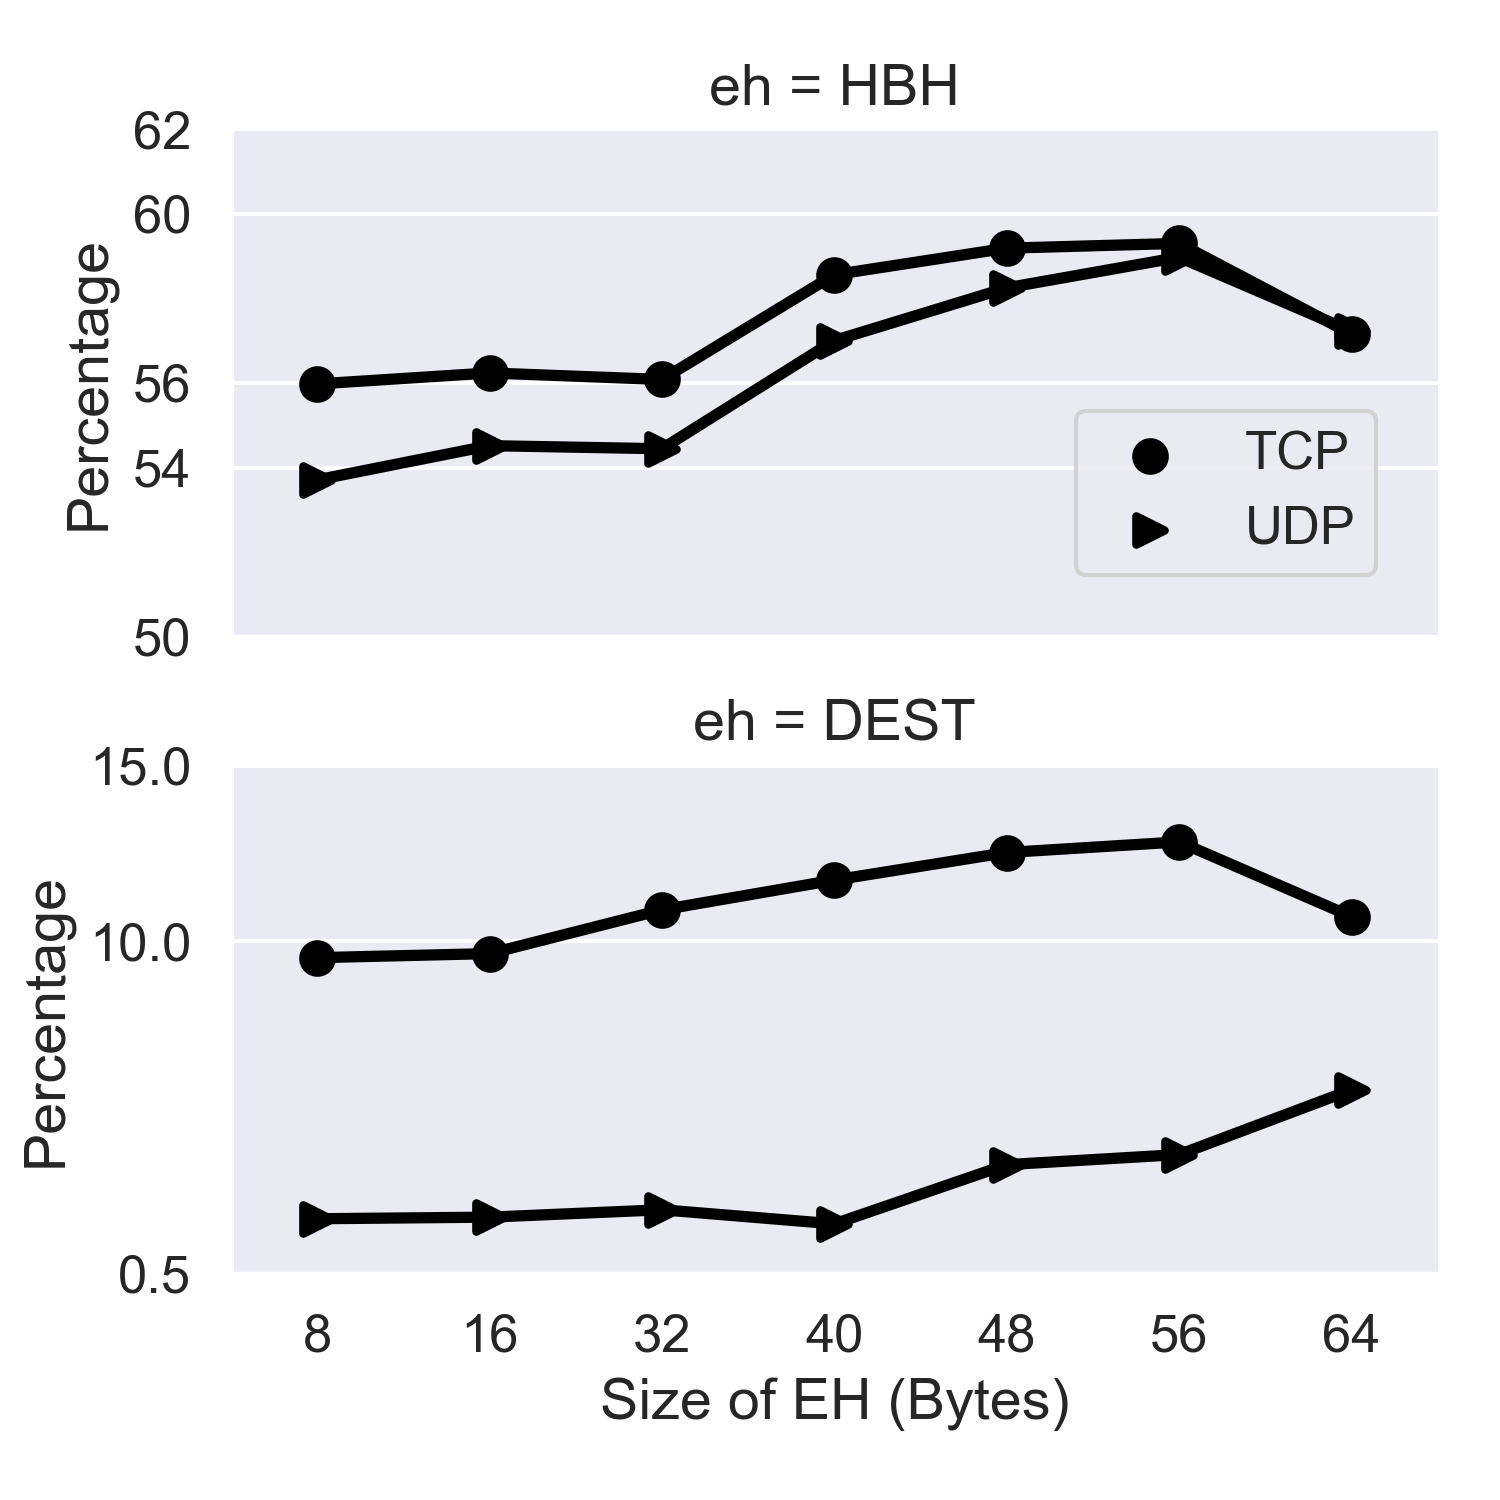
\includegraphics[width=0.5\textwidth]{empty_paths.png}
  \caption{Percentage of paths with drops at the first router.}
  \label{fig:empty_paths}
\end{figure}

Figure~\ref{fig:empty_paths} shows the percentage of
paths where packets are dropped at the first router as a function of the
header size.  
% These are paths where no traceroute response is received for
% test packets including an EH, but responses are received for control packets with no
% EH.
Packets that includes a HBH EH are dropped at the local router for over 50\% of
the paths, whereas a significantly lower drop rate is observed for packets with
DST EHs.  Also, we observe that the type of transport has minimal influence on
the traversal for HBH EHs (54\% UDP, 56\% TCP), but is significant for DST EHs
(2.5\% UDP, 10\% TCP).
The drop rate associated with the header size at the first
router does not display sensitivity to the EH length, compared to that
illustrated in Figure \ref{fig:sizes} for the overall path. A more consistent pattern
 across the entire range of EH sizes is seen,  attributed to the software architecture of
many access routers, which does not have the constriction of a parsing buffer
used in higher-speed routers.

To further understand the impact of the access AS, we examined the
relationship between EH dropping and MSS (Maximum Segment Size) Clamping.
MSS Clamping inserts a TCP MSS Option into the TCP handshake segments
to ``clamp" the MSS for a connection to a suitable value to compensate for
network encapsulation overhead~\cite{custura-mtu}.  
Given that Atlas probes do not send a TCP MSS Option by default, the
presence of an TCP MSS Option at the destination indicates that an intermediate
router inserted it. This implies that router skipped the EH chain to analyse
the complete TCP/IP header to identify the insertion point. If this process
fails, it likely to result in a packet drop.
In our traces, we identified 853 paths to a UK destination where the TCP
MSS option was inserted. Within
this subset of paths, the traversal ratio for HBH EHs is 2.6\%, while for
DST EHs, it is 48.1\%. The chi-square test (p-value$<10^{-43}$) provides
strong evidence of a correlation between EH drops and MSS Clamping, indicating
that drops occur more frequently when MSS Clamping is used. This
problem is likely to reduce when router protocol stacks are updated to support EH. 

\subsection{Effects of Operational Configuration}
    \label{subsec: pathologies}

In some pathological cases, the traversal ratio for packets including HBH EHs is significantly
affected by strict traffic aggregation policies enforced by network operators.
Two notable examples in our traces are the Kazakhstan and Zambian network.
Both destinations are reachable from Atlas only through a single BGP peer
(Border Gateway Protocol). The majority of packets were dropped at the
second to last AS on their path (corresponding to the destination's upstream AS).
While the traversal ratio to the destination's upstream AS shows a behaviour
similar to other destinations (see Fig.~\ref{fig:traversal_pathologies}),
there was a significantly lower traversal ratio to the target AS. This is indicative of a
policy at the tunnel ingress.

% where Hurricane
% Electric (AS6939) serves as the sole BGP (Border Gateway Protocol) peer. This
% network employs a brokering service that tunnels IPv6 peering over an existing
% IPv4 connection to an endpoint situated in Dusseldorf.

Upon closer examination,  nearly all the paths from the
Khazakhstan network that allow a DST EH originate from ASes
located in Australia or New Zealand. Conversely, packets originating from other
geographical areas are filtered at the tunnel endpoint. This is a specific
pathology potentially due to a misconfiguration or policy within this operator's
transit network.
%They can also come from comcast but somehow they bypass HE?!?!?!?!
Similarly, the only BGP peer connecting the target AS in Zambia is Ubuntunet
Alliance for Research and Education Networking.  Notably, there is no shared
origin for the paths where packets successfully traverse from this AS,
indicating that the drops associated with this destination are likely
due to an operator policy. 

These two examples show how configuration and policy 
decisions can result in non-delivery of packets that include EHs, we expect 
that an increase in traffic with EHs could drive resolution of such issues in the longer term.

\begin{table}
\centering
%\caption{Per-AS drop attribution for 8~B DST packets sent from n=4970 Atlas vantage points to a target destination in AS786. The local AS is responsible for the majority (5\% for UDP and 25\% for TCP) of the drops.}
\caption{Traversal Ratios for the ASes along each path}

\begin{tabular}{l|c|c|c|c|c}
   AS     & $1^{st}$  & $1^{st}\rightarrow 2^{nd}$   & $2^{nd}$  & $2^{nd} \rightarrow 3^{rd}$ &   $\infty$ \\ 
\hline \hline
DST UDP  & 95.3\%   & 93\%     &          &          & 91.5\%  \\
DST TCP  & 74.7\%   & 70\%     &          &          & 68.5\%  \\\hline
HBH UDP   & 31.4\%   & 20.1\%   & 15\%     & 12.2\%   & 11.4\%  \\ 
HBH TCP   & 26.9\%   & 16.3\%   & 13.9\%   & 9.7\%    & 8.6\%   \\ 
\end{tabular}
\label{tbl:uk_as1}
%\bigskip

%\caption{Per-AS drop attribution for 8~B HBH packets sent from n=4970 Atlas
%vantage points to a target destination in AS786. The local AS is responsible
%for the majority (68\% for UDP and 74\% for TCP) of the drops.}
%
%\begin{tabular}{p{0.07\textwidth}|l|l|l|l|l}
%
%              & 1st AS & AS1\textgreater{}AS2 & 2nd AS & AS2\textgreater{}AS3 & $inf$     \\ \hline
%HBH UDP & 31.4\% & 20.1\%               & 15\%   & 12.2\%               & 11.4\% \\ \hline
%HBH TCP & 26.9\% & 16.3\%               & 13.9\% & 9.7\%                & 8.6\%  \\ 
%\end{tabular}
% \label{tbl:uk_as2}
\end{table}



%% NB: p-values have been calculated using "scipy" in Python

% observed_DST = [[442, 1124], [411, 2993]]
% observed_HBH = [[883, 728], [15, 3389]]
% chi2, p_value_DST, _ , _ = scipy.stats.chi2_contingency(observed_DST)
% chi2, p_value_HBH, _ , _ = scipy.stats.chi2_contingency(observed_HBH)

% We then look at EH traversal within this subset of paths, to determine whether
% this results in a difference to the overall traversal, on the basis that at
% least one on-path router will have needed to parse the entire IPv6 Header,
% including any EHs, to perform this function.  

\subsection{EHs and Router Forwarding}

Routers using ECMP
(Equal Cost Multi Path) can distribute traffic on different paths based on
a digest that includes the Next Header field (NH) in
IPv6~\cite{lb-classification}, but also can include other fields, such as the 
transport port information. Load-balancing routers can be configured to utlise
layer-3 and layer-4 headers for routing. 
Misinterpreting a NH would result in forwarding
packets of the same flow along a different path solely because it
includes an EH, This could have two implications: It could mean that
the including EH (e.g., to measure a path or to detect a path property)
does not observe the same path. It could also potentially result in
packet reordering within a flow. 
We therefore investigate whether the inclusion of an EH results in a
discernible change in forwarding behaviour compared to packet with no EH.


% The objective of these test was to assess whether routers, which base their
% forwarding decisions on the packet structure, exhibit altered behavior when
% handling packets containing EHs. Our findings substantiate this case,
% highlighting the potential impact of end-to-end use of EHs on network
% utilization.
% 

% Some routers can be configured to select a path based on the Flow Label field
% in the IPv6 header In this case, adding an EH to a packet within a flow would
% not result in reordering.

Paris Traceroute observes the presence of a multipath forwarding by 
performing several measurements between the same
source-destination pair and varying a predetermined set of fields called a
\textit{Paris variation}~\cite{augustin2006avoiding}.  Packets belonging to the
same Paris variation are identified by either a range of sequence numbers in
TCP or the checksum in UDP.

% A router could be designed to use
% various sets of fields for load-balancing~\cite{lb-classification}.

Paris Traceroute was used from the vantage points under our control in Atlas to
the destination in Zambia.  A  particular vantage point was included in this
analysis only if consistently successful in previous tests.  In total, 766
paths were measured.  Each run between a source and a destination pair was
repeated comprised 16 Paris variations, each with a different configuration of
the IPv6 Flow Label and transport port number.  Each variation was repeated six
times to eliminate the possibility that the forwarding path decision was
influenced by an internal source of randomness within the router These same 16
configurations were used in all measurements. 

%Six sets of measurements were run from all vantage points to the Zambian
%destination, with each set of measurement using 16 Paris variations. We select
%the vantage points and destination based on previous measurements, so as to
%only measure complete paths, where traversal always succeeds, 766 paths in
%total.

% The version of Paris Traceroute that was used allowed to deterministically set
% the IPv6 Flow Label and transport port number for measurement in a group of set
% of 16 Paris measurements. The same 16 combinations of IPv6 Flow Label and port
% number were used for subsequent measurement sets.

\begin{figure}[t]
\centering
  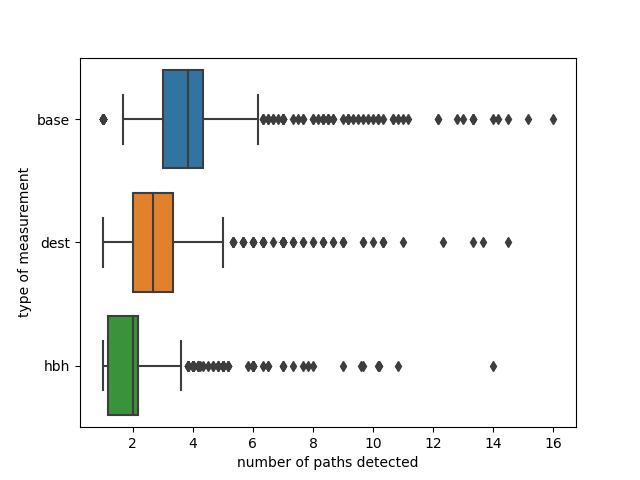
\includegraphics[width=0.5\textwidth]{boxplot-paths-detected.png}
  \caption{Number of paths detected by Paris Traceroute in 866
source-destination pairs, averaged over 5 measurement runs, each using
the same 16 Paris variations. (dataset R3).}
  \label{fig:paths-detected}
\end{figure}

Figure~\ref{fig:paths-detected} compares the distribution of the number of
alternative paths discovered by Paris Traceroute including all
source-destination pairs and Paris variations.  A baseline measurement using packets with no EH
is compared with packets including DST and HBH EHs .  
A median of 4.1 paths in the baseline experiment is consistent with the
results in~\cite{augustin2006avoiding}.  However, when DST EHs and HBH EHs are
included, the median respectively reduces to 2.96 and 2.1 paths.  
% p-value is calculated assuming null hypothesis
This variation in the number of identified paths suggests the inclusion of
an EH influences the forwarding behaviour.  
When analysing individual source-destination pairs, the
measurement with a DST EH detected the same number of paths as the baseline
(within 1 path) in 60\% of cases and fewer paths (by less than 1) in 38\% of
the cases.  The measurement with HBH EHs observed 13.4\%
of source-destination pairs with the same number of alternative paths and
69.7\% having less paths than the baseline.

%%%%%%%%%%%%%%%%%%%%%5

% For some source-destination pairs, the EH Paris measurements detect at least 1
% more path than for a packet with no EH. 
% This below is a bug, I think this is nice for a talk, but awkward for the paper, let's omit
% Although less common (around 1\% of the cases), for specific paths, the introduction
% of an EH resulted in a significant increase in the number of alternative paths,
% far surpassing the count observed without EH.
% For example, in one case, the baseline measurement detected 4 paths, the DST
% measurement found 2 paths, and the HBH measurement uncovered 14 paths. This
% unusual behavior was observed due to a single router exhibiting 14 interfaces
% when handling packets with HBH EHs. While it does not significantly impact
% overall usage, it deviates from expected behavior.

As previously noted, for some source-destination pairs in our dataset, we
observed packet drops when packets included a HBH EH, indicating
inconsistent traversal for packets with this EH. These measurements also reveal
that HBH and DST EH packets are forwarded in the same way as packets without
EHs on only 13\% (for HBH) and 60\% (for DST) of paths.

These results indicate that inclusion of an EH causes some routers to make
different forwarding decisions.  For example, if a simple hash calculation for
path selection that relies on extracting the transport port from a fixed
offset, would fail to provide entropy if it could not correctly locate the port
field. Many routers allow the ECMP information to be calculated in other ways,
e.g. using the IPv6 Flow Label, which would avoid this unfortunate difference
in forwarding.


If the network selects different paths for flows containing EH packets, it
becomes crucial to determine whether these path variations occur within a
single Autonomous System (AS) where consistent configuration policies may be in
place, or across multiple ASes. This distinction is important as it could
result in EH options being processed by different sets of routers than packets
without EH. The implications of this scenario depend on the specific type of
extension being introduced. However, it is important to note that this effect
does not reduce the probability of successful transmission across the path.


%For 12 source-destination pairs in the dataset, not enough data was gathered
%using Destination Option EHs to complete a measurement run. Not enough data
%was gathered for 137 (15.8\%) pairs.

\section{Measuring EH Traversal using PATHspider} 
\label{sec:pathspider-results}
%~\cite{learmonth2016pathspider} 

This section presents results from the analysis of the PATHspider dataset.
These experiments measure the end-to-end traversal from a small
pool of vantage points (5 worldwide locations) to a large number of web and
DNS servers.  Unlike the results based on the Atlas dataset, these
measurement require the server to process the packet containing the EH and
reply.

The IPv6 addresses of the target web servers in these tests were collected by
resolving the domain names in the Cisco Umbrella top 1M list. The IPv6
addresses of the DNS servers, instead, were obtained considering the list of
authoritative name servers for the same list of domains.
Each experiment sent an IPv6 probe packet, either a DNS
query over UDP to a DNS server or a TCP SYN to a web server with a PadN option
included in either a HBH or DST EH, and observed the
corresponding reply.  A test considered the path to support an EH, if a reply was received
both with and without EHs. 

%This section reports the end-to-end support percentage, indicating the paths
%where test packets receive a response from the destination server.

\begin{table} 
\centering
\caption{Server support for DST and HBH EHs (Feb 2023). }
\begin{tabular}{p{1.5cm}|cc|cc}
\multicolumn{1}{l|}{} & \multicolumn{2}{p{2cm}|}{\centering DST support} 
                      & \multicolumn{2}{p{2cm}}{\centering HBH support} \\ \cline{2-5} 
\multicolumn{1}{l|}{} & \multicolumn{1}{c|}{TCP}   & UDP      & \multicolumn{1}{c|}{TCP}     & UDP   \\ \hline \hline
UK                    & \multicolumn{1}{c|}{69.1}  & 69.3     & \multicolumn{1}{c|}{12.5}    & 15.8  \\ \hline
Canada                & \multicolumn{1}{c|}{76.3}  & 76       & \multicolumn{1}{c|}{23.3}    & 24.2  \\ \hline
Australia             & \multicolumn{1}{c|}{72.5}  & 72.2     & \multicolumn{1}{c|}{17.7}    & 17.5  \\ \hline
Singapore             & \multicolumn{1}{c|}{72.8}  & 72.7     & \multicolumn{1}{c|}{17.4}    & 17.4  \\ \hline
Poland                & \multicolumn{1}{c|}{76.5}  & 76.8     & \multicolumn{1}{c|}{24.4}    & 24.7   
\end{tabular}
\label{tbl:e2e_traversal}
\end{table}


\begin{table} 
\centering
\caption{Support for DST and HBH EH from DNS providers (Dec 2022).}
\begin{tabular}{l|c|c|c}
           & \% of dataset &  DST support & HBH support\\
\hline \hline
Cloudflare & 18   & Yes  & No                 \\
\hline
Amazon     & 11   & No   & No                 \\
\hline
Hetzner    & 3    & Yes  & No                 \\
\hline
Gandi      & 4    & No   & No                 \\
\hline
Ionos      & 3    & Yes  & No                
\end{tabular}
\label{tbl:provider_support}
%Google does not support either EH, and is not listed in the table because it was only 30 destinations in the dataset.
\end{table}


\begin{table} 
\centering
\caption{Support for DST and HBH from web providers (Dec 2022).}
\begin{tabular}{l|c|c|c}
           & \% of dataset & DST support & HBH support\\
\hline
\hline
Amazon       & 52                     & Yes                & No                 \\
\hline
Cloudflare   & 23                     & Yes                & No                 \\
\hline
Akamai       & 2.7                    & Yes                & No                 \\
\hline
Google       & 2.3                    & No                 & No                 
\end{tabular}
\label{tbl:web_providers}
\end{table}


\subsection{End-to-end support}
\label{subsec:e2esupport}

Table~\ref{tbl:e2e_traversal} shows the percentage of successful tests to 
DNS servers (UDP) and web servers (TCP). Support for DST EH (69-77\%)  
is higher than HBH EH (12-25\%). These results are only slightly affected by the 
choice of transport protocol,  attributed to the
absence of access routers.

% We find more than two-thirds of Amazon-hosted webservers respond to connections
% by packets including DST, whereas Amazon-hosted DNS servers has no EH support. 

Interestingly, the table also reveals significant variations of the HBH EH
traversal ratio than DST EHs when servers were probed from different vantage
points. For instance, the support for HBH EHs varies from 12\% from a UK
location to almost 25\% from a Polish site.  This indicates that the transit
network may have a greater impact on dropping of HBH EHs than for DST EHs.  

% Overall end-to-end EH
% support for web servers in the dataset range from 72 and 78\% for DST EH and 2
% to 3\% for HBH EH.

%Only one measurement, from the Singapore vantage point, observed a 5\%
%difference based on transport in favour of TCP for both tested EHs. 

The  majority of web servers and at least one-third of the
DNS servers were managed by a few major hosting companies, such
as Cloudflare\texttrademark and Amazon\texttrademark.  Tables
\ref{tbl:web_providers} and \ref{tbl:provider_support} provide a ranking of the
hosting companies based on the share of hosted IP addresses for web and DNS
servers, respectively. The tables also report the policy adopted by these
companies regarding the propagation of packets including DST and HBH EHs.  
This is indicative of how large companies tend to enforce stringent filtering policies to
packets that include EHs, possibly to reduce potential
risks of incorrect handling of EHs.  We found that the policies implemented by
the larger hosting providers have indeed the greatest impact on the global
traversal ratio of packets that include an EH. 

%Our analysis conducted in Feb 2023 found a total of 232,350 IP addresses, the
%majority of which are provided by a few hosting companies: around 52\% of
%destinations were hosted by Amazon Inc, 23\% by Cloudflare, and 2.5\% were
%hosted by Akamai Technologies and Google.  Table~summarises the  EHs for each
%hosting company.

% In order to consider the influence of the major hosting providers,
% Table~\ref{tbl:provider_support} presents the DST and HBH EH support for the
% largest DNS providers in our dataset, along with their incidence.  

To illustrate this impact, consider that in early December 2022, a change of
policy in Cloudflare\texttrademark enabled servers to respond to DNS queries
carrying EHs.  As a result, there was a dataset-wide increase in traversal
from 57\% to 70\%, as currently reported in the table.  Extrapolating from
this, if all the major providers were to enable support, we estimate that the
traversal ratio of this test would exceed 90\% for DST and 60\% for HBH.


\subsection{Analysis of AS support for EHs}

\begin{table}
\caption{Reachable AS by DST or HBH EHs (Dec 2022).}
\begin{tabular}{l|c|c}
Supported EH                & Paths per AS$>$=1 & Paths per AS$>$=10 \\
\hline \hline
Total  ASes                 & 2787              & 1606 \\
\hline
%No DST support             & 212 (7.6\%)        & 110 (6.8\%)    \\
DST on at least 1 path      & 2575 (92.4\%)     & 1496 (93.2\%)      \\
DST on at least 50\% paths  & 2476 (88.8\%)     & 1437 (89.4\%)      \\ \hline
%AS does not support HBH  & 1287 (46.2\%)  & 709 (44.1\%)            \\
HBH on at least 1 path      & 1500 (53.8\%)      & 897 (55.9\%)      \\
HBH on ar least 50\% paths  & 1037 (37.2\%)      & 580 (36.1\%)  
\end{tabular}
\label{tbl:as_pathspider}
\end{table}

If we consider the traversal of EHs in target ASes rather than to individual
servers, the outlook is different.  Table~\ref{tbl:as_pathspider} reports the
number of ASes containing the target DNS servers that could be reached from at
least one vantage point over at least one path and compares this with the total
number of ASes (2nd column) discovered in the trace. To assess that this
metric is valid across multiple paths to the AS, we also report the number of
ASes reachable over a least 10 paths (3rd column), and those that succeed in more
than half of paths in both DST and HBH cases (3rd and 5th row, respectively).
These estimates of the actual support of EHs in ASes
are conservative, because a destination ASes not reachable from any
vantage point could be masked by upstream ASes that dropping EHs.

%Tablepresents the traversal
%rates for the ASes targeted by PATHspider (2868 in total). 

% from at least one of the vantage points.
% a target server belonging to the AS probed f
% The first column considers all destination ASes in the dataset, while the
% second only looks at ASes that host 10 destination addresses or more. 


% alongside evidence that they support either the DST or HBH EH.  If at
% least one reply is seen from an AS to one of our test packets from any of the
% locations tested, we consider that AS supports the traversal of packets that
% include the tested EH type. 

The results highlight that most (90\%) of ASes forward packets that include an  8~B DST EH
 and about half forward packets with an
8~B HBH EH.  There is little variation when considering the ASes (1606) tested over 10 or more paths.  
This suggest that DNS servers are often have
ASes with stricter policies.

The traversal reduces for packets that travel to the destination
through multiple ASes, suggesting that many packets  could be
dropped before reaching the destination AS. For DST, 3.4\% fewer ASes
allow DST traversal on more than half the paths, whereas for HBH, the
difference is 16.6\%. Again, this demonstrates the need for  transit 
networks to support HBH EHs. 

\subsection{Support for IPv6 Options}

\begin{table}[t]
\centering 
\caption{Support for EH Options in DNS queries.}
\begin{tabular}{l|c|c}
Test                      & DST support & HBH support\\
\hline \hline
Pad N Option (1)          & 69.3        & 15.1       \\
PMTU Discovery (48)       & 69.5        & 15.8       \\
Experimental Option (30)  & 69.4        & 15.1       \\
Experimental Option (254) & 0.4         & 0          \\
Incorrect Option Length   & 0.5         & 0.05            
\end{tabular}
\label{tbl:option_type_support}
\end{table}

Measurements were performed to determine whether the results are 
influenced by option data carried in the EH.  We first
evaluated the effect of the two higher ordered bits of the option type
that indicate how router should behave when the option is unknown~\cite{rfc8200},.
Table~\ref{tbl:option_type_support} reports the percentage of support for various
option types in tests towards DNS servers.  In addition to the already
considered PadN Option, we tested the recently standardised MinPathMTU
HBH~\cite{rfc9268}, and two experimental options: 30 and
254~\cite{RFC4727}.  The latter are specified for testing
only,and are ought to be dropped by all routers, since the two most
significant bits are set.  

The measurements show that if when two most significant bits are unset (i.e. option type
$\le 63$), the type of option has no affect on EH support, because traversal 
is similar in all cases. When the highest order bits are set, the
packet was expected to be dropped~\cite{RFC8200}.  Instead, we receive
responses for 0.4\% of paths. This means that these bits have been ignored by all
routers on a small number of paths.
Finally, we tested an incorrectly set Option Length field. Any node parsing
this EH field should validate the Option Length and discard the
packet~\cite{RFC8200}. However, also in this case, we also found a small number of
paths (0.5\%) where all routers on the path ignore the field. We suggest
these routers could have been configured to ignore the EH~\cite{RFC8200}.

\begin{table}[t]
\centering
\caption{Percentage of Probes Triggering ICMP messages.}
\label{tbl:icmp_support_dst}
\begin{tabular}{l|p{0.04\textwidth}|
p{0.03\textwidth}|p{0.03\textwidth}|p{0.03\textwidth}|p{0.03\textwidth}|p{0.025\textwidth}}
                           &          & UK        & Can       & Aus    & Sgp          & Pol     \\
\hline
\hline
{ICMP rcvd from local AS}  & {HBH DST} & {0 100}  & {0 51.6}    & {0 51.9}    & {0 51.9}    & {0 51.5}  \\
\hline
{ICMP rcvd from other AS} & {HBH DST} & {72.8 0} & {52.5 0}    & {68.2 0}    & {69.2 0}    & {73  0}   \\
\hline
{ICMP rcvd \& packet fwd} & {HBH DST} & {0 0.52} & {0 0.48}    & {0 0.46}    & {0 0.24}    & {0 0.46}  \\
\hline
{ICMP not received}        & {HBH DST} & {27.2 0} & {47.5 48.4} & {31.8 48.1} & {30.8 48.1} & {27 48.5} 
\end{tabular}
\end{table}


\subsection{ICMP Parameter Problem Messages}

% When a packet includes a DST or HBH Option with the two MSBs set, a router
% that does not recognise the Option should discard the packet returning an
% ICMP \textit{Parameter Problem} message to the sender~\cite{RFC8200}. 
% Results for DST and HBH are presented in Table~\ref{tbl:icmp_support_dst}.  

A router unable to process an option with a non-zero value
for the MSBs ought to return an ICMP message.
Option type $\ge 192$ should cause the packet containing the Option to be discarded and
return an ICMP "Parameter Problem" message~\cite{RFC8200} to the source.
This behaviour was  observed from the all the vantage points, beacause the
first router on the path, the local router, returned an
ICMP message for a packet including a DST EH containing Option 254
(Table~\ref{tbl:icmp_support_dst}).  However, only between 50 and 100\% of
probes depending on the vantage point generated an ICMP.
An ICMP return ratio lower than 100\% should be attributed to ICMP
rate-limiting mechanism.  The same
rate-limiting was also observed for ICMP message generated by other routers
 in response to HBH EHs with Option 254.  The widespread presence of
rate-limiting makes the use of ICMP notifications an unreliable
indicator of packet drops due to an unknown Option.

In a minority of cases, we encountered paths where packets were consistently
forwarded regardless of the MSB settings, or instances (0.2-0.5\% of paths
using DST) where an ICMP message
was generated and the packet was still forwarded to the destination.

% This suggests that certain routers deviate from the RFC 8200 specifications,
% indicating a lack of proper adherence to the standards.

\subsection{ICMP Destination Unreachable}

When a packet is discarded due to an EH, an ICMP "Destination Unreachable"
message could be generated back to the sender.
We found that for all destinations, an ICMP
"Destination Unreachable" message is received in up to 2\% of the path
even if the test succeeds.  For tests with a
HBH EH over paths towards DNS servers, the ICMP messages
are only returned for 0.2\% of the paths. For packets including DST, these messages
are also infrequent, ranging from 0.3 to 8.8\% of paths depending on the
vantage point. 
This indicates that ICMP messages cannot be reliably used to
determine whether a packet was dropped in transit due to the presence of Options.
In this cases, ICMP messages are exclusively received from
routers in destination ASes and are a result of an incorrect processing of the
EH~\cite{RFC8200}.


\subsection{Longitudinal Analysis of Support for EH}

Table~\ref{tbl:longitudinal_support} shows a longitudinal analysis
across a set of domains collected over 3 years,  between Jan 2020 and
Dec 2022.  The table shows support for an 8~B Pad N Option for both DST and
HBH EHs, from a single vantage point to the authoritative NSes for the dataset P1.
Each tested domain was resolved at the time of the measurement, resulting in a
different pool of IP addresses in each session. 
This shows a trend for decreasing support of HBH. However, the DST support
remained constant until December 2022 when Cloudflare\texttrademark enabled support on
their network boosting  overall support, as previously
mentioned in Section~\ref{subsec:e2esupport}.

% Ana: verify total number of paths.
\begin{table}
\caption{Support for an PadN Option for DST and HBH EHs towards DNS servers.}
\begin{tabular}{l|c|c|c|c}
              & Jan 2020 & Jul 2020 & July 2022 & Dec 2022 \\
\hline \hline
DST support   & 59.9\%   & 54.3\%   & 57.4\%    & 71.7\%   \\
HBH support   & 25.7\%   & 23.8\%   & 16.4\%    & 11.9\%   \\
\hline
Unique IP addresses & 18296    & 19690    & 19553     & 20050   
\end{tabular}
\label{tbl:longitudinal_support}
\end{table}


\section{Discussion} 
\label{sec:discussion}

Since its standardisation, the IPv6 protocol has
seen widespread adoption~\cite{v6adoption_ton} and the hardware and software that
support it have also matured: packet parsing capability in routers is improving and
router architectures have continued to evolve~\cite{metamorphosis, hauser2023}, including some designs based on hardware and re-configurable
logic enable new functions to be introduced~\cite{cisco-silicon-one}. Updates  have also been made to the IPv6 standard based on operational experience~\cite{RFC5722}~\cite{RFC6946}~\cite{RFC6564}~\cite{RFC8200}.
The next sections discuss the usability EHs on Internet paths and the barriers to introducing new options.

\subsection{Usability of EH across Internet Paths}

EH processing has become a recent focus in the standards community~\cite {ietf-v6ops-hbh-03}, where new applications are emerging. Many current deployment scenarios are within a single domain. There are proposals to help facilitate an increase in support for EH~\cite{ietf-6man-HBH-processing-06, ietf-6man-eh-limits-02}. 
So, it is timely to ask what is the prospect for using EHs to extend IPv6 across adjacent domains across end-to-end Internet paths?

First, we consider whether a packet including an EH is expected to traverse an Internet path.
We find that packets that include the DST EH traverse up to 96\% of Internet paths~\ref{fig:countrybox} and that over 92\% of server edge ASes~\ref{tbl:as_pathspider} also support DST.


We also find that packets that include HBH EH are supported on paths from some vantage point. For many transit network these are dropped  (Table~\ref{tbl:as_pathspider}) and also by many access networks (see Figure~\ref{fig:countrybox}). Mis-configuration or other network policies also result in various pathologies within transit networks, shown in Subsection~\ref{subsec: pathologies}. 

We also find that traversal reduces significantly for packets that include EHs (both DST and HBH) when a path contains edge-network routers that insert a TCP transport option, and infer that resolving this likely requires updates to these routers.

Server-side, testing the same set of name servers between 2019 and 2022 reveals the support for 8~B PadN HBH has decreased over time when considering individual destinations (Table~\ref{tbl:longitudinal_support}), because servers have become more centralised under only a few ASes that do not support HBH.  However, an analysis by AS results reveals more than half of the tested ASes allow packets that include a HBH EH. This confirms that transit networks can present an still obstacle to use of the HBH EH.

RFC 7872~\cite{RFC7872} describes the traversal to the authoritative name servers for the Alexa Top 1M domains in 2014. This observes packets including an 8~B PadN DST traverse paths to 78.6\% of server destinations and packets including an 8~B PadN HBH traverse paths to 45.9\% of destinations. These results were measured from a single vantage point and are not grouped per AS, and therefore can only be compared with results in Table~\ref{tbl:longitudinal_support}. The comparison indicates a 5-9\% decrease in support for DST and a 25-30\% decrease in support for HBH, although we note this could reflect the choice of vantage point or changes within the top 1M domain list itself between 2014 and 2023.
The AS analysis reveals that packets that include an EH traverse to up to 90\% and over 50\% of ASes respectively. This hows a decrease is due to drops within the destination AS.
To understand if traversal can be improved by limiting the size of the total EH Chain, we explored using different size of EHs and found that EH chains of up to 40~B have a higher probability of traversing an access network path with a UDP transport, shown in Figure~\ref{fig:sizes}.

XXX This result ought to be true of HBH options also - but care has to be taken to only check HBH EH size when the path supports a HBH extension header XXX
This suggests that when using EHs, keeping the packet size under this limit would help in ensuring consistent deployment.

%Question 2: is there a limit to extension headers that prevents them from traversing certain Internet paths such as limiting length of the EH chain or a specific EH length? Would ? Is it different between HBH and DO?

%XXX Do we have a short statement on use between a set of adjacent transit domains? XXX

In some cases, low traversal was attributed policy-based dropping. While configured ACLs may be necessary in some networks today to protect routers (e.g. where EH processing cannot be disabled and leads to DoS vulnerabilities or undesirable side-effects~\cite{passive-threats}). In cases where this is not needed, such a policy is not desirable, because it results in ossification that will obstruct new uses of EHs.

% XXX A way forward is to skip the EH to facilitate HBH support and still protect the control plane

% makes sense to use them within domains, where encryption is not needed, but perhaps in an 'untrusted' domain quic etc is better


%Question 6: what is the opportunity for destination options? Is it a good trade-off to have a network layer? That is consistent transport header or is it wiser to put the transport header information within the transport and therefore allow it to be encrypted such as quic transport parameter - so what is the real advantage of destination options?


%Question 3a: When options extension headers do traverse, do they traverse consistently for the same pair of endpoints?

%Quetsion 3b: Does the Flow Label help to ensure a consistent set of network routers on a path? -- If not, then we ought to suggest the step towards evolution would be to add a PAD option to all packets that would not otherwise have an EH?
%Question 3c: Is there a trend to set meaningful entropy in the Flow Label against the original place where many endpoints sent a zero value Flow Label?
%Question 3d: Is the Flow Label invariant .... is the FL the same at src as at the dst ...  (i.e. do devcies on-path rewrite) is that something RIPE could easily answer. - If they reset to zero then they are evil!
%Here we should not forget the proposals to add flow metadata as a hop by hop extension to let network routers know helpful information to help forwrad the packets in a flow.

%Question 5: If we find HBH don’t work everywhere then ….What is the opportunity for using a hop by hop extension header on some of the packets belonging to a flow? does this result in new forwarding pathologies? That is where the packets that include EHs take a different set of routers to the packets with no extension headers, and if so do they take a different network or do they simply follow a different path through the same operator network? Does this result in inconsistent loss? Is the option useful ?

Our experiments also varied both the Flow Label and the source port of packets to detect if the inclusion of a DST or HBH EH in a packet influenced the path between the endpoints. Results presented in Figure~\ref{fig:paths-detected} show that this inclusion can change a packet's forwarding path. We attribute this discovered variation to the position of the EH between the IPv6 header (which contains the Flow Label) and the transport header (which contains the transport port), suggesting some load-balancing network equipment does not process or skip the header chain to find the actual port information, but might instead wrongly use a byte offset to the expected position of the source port. Overall, this shows traffic flows that use a mix of packets that include an EH and packets without, must take care as these packets may not travel on the same Internet path, resulting in reordering or differences in patterns of loss/delay. 
This motivates the use of Flow Label for load-balancing~\cite{RFC6437}. However,  the flow label has also been re-used for various purposes~\cite{flow-label-approaches} including mobility, traffic engineering~\cite{traffic-eng} and load-balancing. Some routers already use the Flow Label to perform load balancing~\cite{lb-classification}. Modern operating systems set the Flow Label on packets in the same traffic flow~\cite{os-fl}. We argue following the recommendation in~\cite{RFC6437} would mitigate the need to parse the entire IPv6 header chain by load-balancing devices, and would also prevent reordering where packets including an EH are part of the same flow as packets without EHs, enabling new use-cases. 


%Who sets the flow label???


\subsection{Potential to Introduce New Options}

We next determine whether new options could be defined and used across the Internet.
Our  data  shows that packets including DST can already traverse many paths both across the core of the Internet, and at the server and network edge. 
We find that traversal does not depend on the type of Option  (see Table~\ref{tbl:option_type_support}). This is important because it suggests a new DST or HBH Option can be defined and then used on any path that allows EH processing. 
As the functionality to process a new HBH Options needs to be implemented in routers, we suggest it is unlikely that all routers on an Internet path will support a specific HBH Option. Therefore, we recommend that any functions that use an Option need to be designed to be robust to routers skipping HBH processing (e.g., the MinPMTU  Option~\cite{rfc9268,rfc9343}). 

% When evaluating traversal of a DST Option with both its two MSBs set, and which was unknown to routers on the path, our results show that most routers are currently configured to discard packets and to send an ICMP message, as specified by~\cite{RFC4443}. However, we did find some instances where the router (correctly) sends an ICMP message in response to a DST EH including this Option, but nevertheless forwarded the packet; more commonly, packets that include a HBH Option with both MSBs set are forwarded (without sending an ICMP message). When considering whether or not a new Option needs to set its two MSBs, protocol designers should take into account that ICMP was not found to be a reliable mechanism for indicating whether a path implements a new function.

Since ~\cite{rfc2460}, there have been important changes in the way that EH are used - i.e. routers only processing these when support is explicitly configured, impacts the usefulness of the ICMP messages. We also note that it is no longer expected ICMP messages are delivered across paths, and therefore an endpoint can't rely on ICMP messages to infer whether functions are supported, and instead advocate a happy eyeballs approach to race packets with and without EH.

%\subsection{Potential to incrementally extend IPv6}

Whereas, the inclusion of a HBH EH has only recently starting to be used and has motivated the implementation of router architectures that can offer hardware processing. This has motivated interest by the standards community~\cite{ietf-6man-HBH-processing-06, ietf-v6ops-hbh-03, ietf-6man-eh-limits-02} and is expected to help foster development of new Options and motivate support by network operators. When we considering inclusion of an EH, we conclude that Internet successful traversal needs to take into account the type of network path.

We suggest it is possible to incrementally extend IPv6 by only including an EH when a path is found to be supported,
suggesting a method similar to ~\cite{rfc9268}:
An application can be designed to first send a test packet including an EH with the required Option, or combination of Options, and not send additional packets that include this EH until the test packet is acknowledged. The process of sending packets both with and without a header to discover whether a path can support that specific header is sometimes called ``racing" (e.g., transport protocol racing is explained in~\cite{ietf-taps-arch-18}; this resembles ``A/B protocol feature testing", as used in Pathspider~\cite{learmonth2016pathspider}). Our results show that for up to 3 quarters of access networks, the first AS on the path will drop packets including HBH (Table~\ref{tbl:uk_as1}. In this case, racing would not discover a path where this EH is supported. However, on the remaining ~1335 access networks, our results show that depending on the destination, racing would find between at least 31\% paths (in the case of UK destination) and 66\% (in the case of Zambian destination) supporting them.
This could also be used to extend methods currently restricted to controlled domains (e.g.,  within an AS), could in future be used to extend IPv6 (e.g., to enable performance measurement and management ~\cite{rfc8250}~\cite{ietf-ippm-ioam-ipv6-options-10} across consecutive multiple domains).
Since the set of routers forming a path can change with time, this discovery process ought to be repeated from time-to-time. 

 
\section{Conclusion}
\label{sec:conclusion}

This paper presents new results exploring the traversal of packets that include a HBH or DST EH, measured across Internet paths, seeking to answer the question of whether EH can be used to extend IPv6 functionality. This is the first detailed study to include not just end-to-end traversal, but also to consider the treatment by the routers along the path. Our results consider both access and transit networks

The probability of successful traversal of a packet can depend on the type of included EH, the size, and also on the transport protocol carried in the packet payload. The end-to-end traversal is also function of the type of network(s) forming the path, that is, it is strongly influenced by the location of the source and destination. Results are therefore presented from a range of vantage points.
These results demonstrate that if the EH chain is currnetly limited in size (e.g. less than 40~B), packets including a DST EH can traverse as many as
95\% of a diverse set of Internet paths. While packet that include a HBH EH only traverse a narrow set of paths. They often fail to traverse the local access network, although in some cases they are dropped by an AS further along the path. When we characterise whether packets traverse an AS and exclude operator policies in access and transit networks, we find many ASes do forward packets that include this type of EH.

Our results also
demonstrate that the inclusion of some EHs in packets on paths with network layer load-balancing often results in a narrower set of forwarding paths. 
This  could be eliminated by utilising the IPv6 Flow Label, or ensuring that routers using ECMP are able to traverse the entire IPv6 header chain. The implications of this will depend on the type of extension being introduced. Importantly, this effect did not reduce the reduce the probability of successful transmission across the path.

In summary, these results suggest there are  opportunities to use IPv6 HBH and DST EH beyond a single controlled domain, with the expectation that applications incrementally utilise new features using HBH and DST EHs. We  provide recommendations for the design of new features using Options. These need to consider that not all routers process EHs and that some paths drop packets that include EHs. To overcome these deployment challenges, we motivate the use of racing methods to facilitate incremental deployment, which could be deployed to enable new IPv6 functionality (in this case to improve detection for support for larger sizes of packets). Similarly, we suggest that methods currently restricted to controlled domains (e.g., within an AS), could in future be used to extend IPv6 (e.g., to enable performance measurement and management across multiple domains).

\section*{Acknowledgements}

The authors appreciate the valuable comments provided by Justin Iurman and Benoit Donnet and Eric Vincke. This work has been partially supported by the University of Aberdeen's School of Engineering Department, and experiments using ATLAS probes were funded by the RIPE
NCC Community Fund, Project ID 619935.

\bibliographystyle{abbrv}
\small
\bibliography{main,rfc}


\end{document}
